% Drawing 98/02-1 -- folder 98, batch 02, archive page 28 (PDF page 29).
% Transcription: dans la marge gauche, au crayon, un petit croquis : une nappe en parallélogramme marquée $X$, traversée de trois traits dans le sens de sa hauteur et de courts traits épais dans l'autre sens, avec $K'$ près de son bord inférieur et $S$ à son coin supérieur droit ; à gauche, une verticale ponctuée de petites boucles descend jusqu'à un $S$.
% Kind: sheet (parallelogram) over a base line, with fibres. Method 2 (schematic redraw from the facsimile). Status: ok.
% Notes: Left margin, faint pencil. A tilted sheet (X): upper, right and lower sides in pencil, the left side a heavy stroke carrying a small cross; three lines across it, roughly parallel to its right side, the first starting below the upper side as on the page; eight short heavy strokes across these lines (on the upper side, in the middle and on the lower side); the letter X inside, K' near the lower side, S beside the upper right corner; from the lower left corner a loop going down to the left; at the far left a long vertical line in a brownish ink with small curls along it, ending at a letter S. Still differs: the pencil is faint and the sketch crowded; the heavy cross strokes are placed by eye and their number is a reading; the small curls on the vertical are drawn as short ticks; what the cross strokes stand for (the points over K_1, K_2?) is not settled. Nothing struck. The long vertical stroke to the right of the sketch borders the definition and is not drawn. Overlaid 2026-11-12 (Opus 5.5) on a 400 dpi colour render: the left side had been closed as a pencil edge some 4 to 6 units right of the heavy stroke that forms it on the page, which was missing; the first cross line started on the upper side, 13 units too high; the loop at the lower left was too narrow; one cross stroke was 4 units off; corrected. Redrawn 2026-11-12 (issue 128): to check again. 2026-11-13, Claude Opus 5.5, overlay check (issue 147): not compiled (no TeX in the session); the TikZ rasterised and laid over the 350 dpi colour render of the scan, with an ink/pencil separation of the crop, which makes the faint pencil legible. Redrawn on the ink: the sheet is open, not a closed parallelogram: the upper side runs to the top corner, the right side comes down from it only to about y = 35, the lower side runs from the heavy stroke at the lower right to the lower left corner, and the left side is the heavy stroke with its small cross; the second and third lines across were 4 to 15 units off (the second starts below the X, with a faint fragment near the upper side; the third is a heavy stroke from (74.3, 32.7) to (79, 62.5), with a separate thin stroke near the top corner); nine short heavy strokes across, each on its ink, with the small pencil curl before the one on the right and two pencil strokes; the far-left vertical in brown ink with its loop at the top and its three curls drawn as curls (they were ticks); the loop at the lower left and the labels X, K', S and S on their ink. Every element lies on the ink to within about 1 unit. Left out, as before: the long vertical stroke at the right, which borders the definition. What the cross strokes stand for is a question of reading, not of the drawing.
% Coordinates: 1 unit = 1 mm = 1/100 of the crop width (bbox in page fractions: [0.1, 0.2, 0.24, 0.33]).
% Redrawn by Claude (claude-fable-5-2), issue #128, 2026-11-12; not checked by a human; not compiled (no TeX in the session).
% Overlaid by Claude (claude-opus-5-5) 2026-11-12 (issue #128): rasterised from its own coordinates over the colour facsimile and checked or corrected. Not compiled. Status: partial.
% Revised by Claude Opus 5.5 (claude-opus-5-5), issue #147, 2026-11-13: overlay check on the colour scan; not checked by a human; not compiled (no TeX in the session).
% Rights: reproduces part of the work -- behind RENDER_TRANSCRIPTS, never published by itself.
\documentclass[tikz,border=3pt]{standalone}
\usepackage{amsmath,amssymb}
\usetikzlibrary{patterns,arrows.meta}
\tikzset{pencil/.style={black!45}, struck/.style={black!35}, mpt/.style={circle,draw,inner sep=1.3pt}, pt/.style={circle,fill,inner sep=0.9pt}, opt/.style={circle,draw,fill=white,inner sep=1.1pt}, Br/.style={brown!70!black}}
\begin{document}
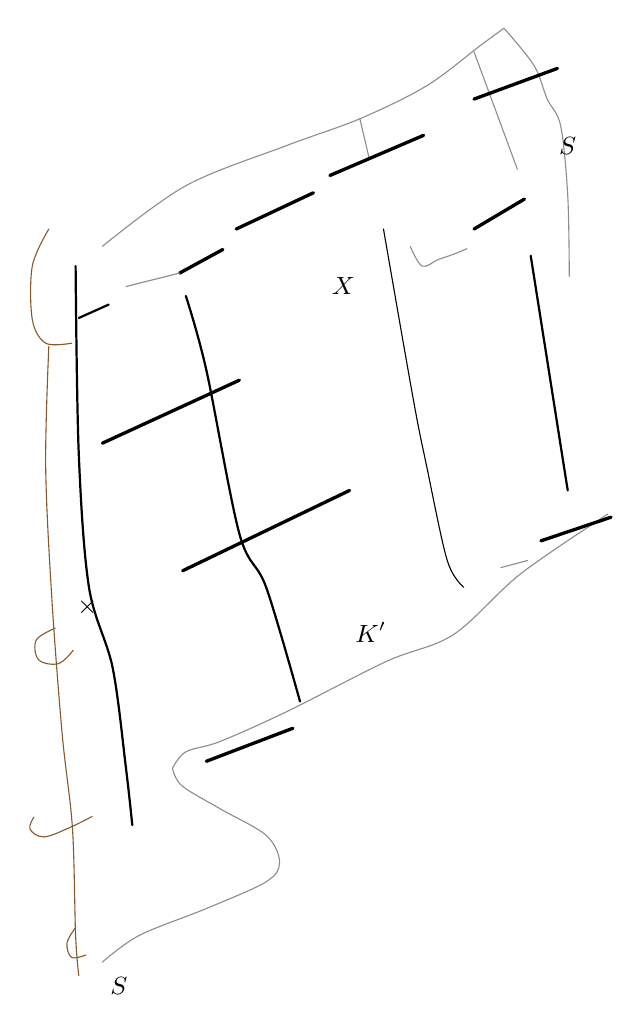
\begin{tikzpicture}[x=1mm,y=1mm,line cap=round,line join=round,font=\small]
% the sheet: upper side, right side (open below), lower side (pencil), left side (a heavy stroke with a small cross)
\draw[pencil] plot[smooth, tension=0.55] coordinates {(19.9,-31.5) (30.5,-23.8) (43.3,-18.7) (52.6,-15.3) (61.1,-11.1) (67.9,-6) (70.9,-3.8)};
\draw[pencil] plot[smooth, tension=0.55] coordinates {(70.9,-3.8) (74.7,-8.5) (76.4,-12.8) (78.1,-16.2) (79,-25) (79.2,-35.3)};
\draw[pencil] plot[smooth, tension=0.55] coordinates {(84.1,-65.5) (73,-73.1) (64.5,-80.8) (56,-84.2) (43.3,-90.6) (34.8,-94.4) (30.5,-95.7) (28.8,-97.8)};
\draw[thick] plot[smooth, tension=0.55] coordinates {(16.5,-34) (16.9,-57.8) (18.2,-74.8) (21.2,-85) (22.9,-97.8) (23.7,-105)};
\node at (18,-77.3) {\small $\times$};
\draw[thick] (16.9,-40.6) -- (20.7,-38.9);
% the loop from the lower left corner down to the left
\draw[pencil] plot[smooth, tension=0.55] coordinates {(28.8,-97.8) (30,-100) (34.8,-102.9) (40.7,-106.3) (42.4,-109.7) (40.7,-112.2) (33.1,-115.6) (24.6,-119) (19.9,-122.4)};
% three lines across the sheet (the second with a faint fragment near the upper side), and a thin stroke near the upper right corner
\draw[thick] plot[smooth, tension=0.55] coordinates {(30.5,-37.8) (33.1,-47.2) (37.3,-68) (40.7,-74.8) (45,-89.3)};
\draw plot[smooth, tension=0.55] coordinates {(55.6,-29.3) (59.4,-51) (61.1,-59.5) (63.7,-71.4) (65.8,-74.8)};
\draw[pencil] (52.6,-15.3) -- (53.8,-20.4);
\draw[thick] (74.3,-32.7) -- (79,-62.5);
\draw[pencil] (67.1,-6.8) -- (72.6,-21.7);
% the short heavy strokes across
\draw[very thick] (67.1,-12.8) -- (77.7,-8.9);
\draw[very thick] (48.8,-22.5) -- (60.7,-17.4);
\draw[very thick] (36.9,-29.3) -- (46.7,-24.7);
\draw[very thick] (29.7,-34.9) -- (35.2,-31.9);
\draw[pencil] (22.9,-36.6) -- (29.7,-34.9);
\draw[very thick] (67.1,-29.3) -- (73.5,-25.5);
\draw[pencil] plot[smooth, tension=0.6] coordinates {(59,-31.5) (60.5,-34) (62.5,-33.2) (64.5,-32.5) (66.2,-31.8)};
\draw[very thick] (19.9,-56.5) -- (37.3,-48.5);
\draw[very thick] (30.1,-72.7) -- (51.3,-62.5);
\draw[very thick] (33.1,-96.9) -- (44.1,-92.7);
\draw[very thick] (75.6,-68.9) -- (84.5,-65.9);
\draw[pencil] (70.5,-72.3) -- (73.9,-71.4);
% labels
\node at (50.5,-36.5) {\small $X$};
\node at (54,-80.5) {\small $K'$};
\node at (79,-18.8) {\small $S$};
% at the far left, the long vertical in brownish ink, its loop at the top and the curls along it, down to S
\draw[Br] plot[smooth, tension=0.55] coordinates {(13.1,-29.3) (11,-34) (11,-40.8) (12.7,-43.8) (16,-43.8)};
\draw[Br] plot[smooth, tension=0.55] coordinates {(13.1,-44.2) (12.7,-59.5) (13.5,-76.5) (14.8,-93.5) (16.1,-105.4) (16.5,-119) (16.9,-124.1)};
\draw[Br] plot[smooth, tension=0.6] coordinates {(13.9,-80) (11.5,-81.5) (11.8,-84) (14.3,-84.5) (16.2,-82.8)};
\draw[Br] plot[smooth, tension=0.6] coordinates {(18.6,-103.9) (16,-105.2) (12.5,-106.5) (10.7,-105.5) (11.2,-104)};
\draw[Br] plot[smooth, tension=0.6] coordinates {(16.5,-118) (15.4,-120) (16,-121.8) (17.8,-121.5)};
\node at (22,-125.4) {\small $S$};
\end{tikzpicture}
\end{document}
